%%%%%%%%%%%%%%%%%%%%%%%%%%%%%%%%%%%%%%%%%%%%%%%%%%%%%%%%%%%%%%%%%%%%%%%%%%%%%%%%
\chapter{Future Work}\label{ch:future-work}
%%%%%%%%%%%%%%%%%%%%%%%%%%%%%%%%%%%%%%%%%%%%%%%%%%%%%%%%%%%%%%%%%%%%%%%%%%%%%%%%

%%%%%%%%%%%%%%%%%%%%%%%%%%%%%%%%%%%%%%%%%%%%%%%%%%%%%%%%%%%%%%%%%%%%%%%%%%%%%%%
\section{Future Work's table}

On the table~\ref{tab:future-works} we list a set of ideas of future works. The sections A to D comprehends topics on the evolution of SIMITAR. Section E mentions new ideas of research that can contribute to SIMITAR evolution, but are not restricted to. Also, some topics can be a starting point for new tools.


\begin{table}[!ht]
\centering
\caption{Future Work's table}
\label{tab:future-works}
\begin{tabular}{lll}
\hline
\rowcolor[HTML]{9B9B9B} 
\multicolumn{1}{c}{\cellcolor[HTML]{9B9B9B}A} & \multicolumn{2}{l}{\cellcolor[HTML]{9B9B9B}Performance}                                                         \\ \hline
                                              & 1                          & Modeling Optimizations                                                             \\
                                              & \cellcolor[HTML]{EFEFEF}2  & \cellcolor[HTML]{EFEFEF}TinyFlows and flow merging                                 \\
                                              & 3                          & Smarter Flow Scheduler and thread management                                       \\
                                              & \cellcolor[HTML]{EFEFEF}4  & \cellcolor[HTML]{EFEFEF}DPDK KNI Interfaces                                        \\
                                              & 5                          & Multi-thread C++ Sniffer                                                           \\ \hline
\rowcolor[HTML]{9B9B9B} 
B                                             & \multicolumn{2}{l}{\cellcolor[HTML]{9B9B9B}Tool Support}                                                        \\ \hline
                                              & 1                          & Inter-packet times on TinsFlow                                                     \\
                                              & \cellcolor[HTML]{EFEFEF}2  & \cellcolor[HTML]{EFEFEF}D-ITG Flow Generator: DitgFlow                             \\
                                              & 3                          & DPDK Flow Generator: DpdkFlow                                                      \\
                                              & \cellcolor[HTML]{EFEFEF}4  & \cellcolor[HTML]{EFEFEF}Ostinato Flow Generator: OstinatoFlow                      \\
                                              & 5                          & ZigBee protocol Support                                                            \\ \hline
\rowcolor[HTML]{9B9B9B} 
C                                             & Calibration                &                                                                                    \\ \hline
                                              & 1                          & min\_time                                                                          \\
                                              & \cellcolor[HTML]{EFEFEF}2  & \cellcolor[HTML]{EFEFEF}min\_on\_time                                              \\
                                              & 3                          & session\_cut\_time                                                                 \\ \hline
\rowcolor[HTML]{9B9B9B} 
D                                             & \multicolumn{2}{l}{\cellcolor[HTML]{9B9B9B}New Components}                                                      \\ \hline
                                              & 1                          & Traffic Measurer                                                                      \\
                                              & \cellcolor[HTML]{EFEFEF}2  & \cellcolor[HTML]{EFEFEF}Pcap files crafter                                         \\
                                              & 3                          & Python/Lua Flow Generator                                                          \\ \hline
\rowcolor[HTML]{9B9B9B} 
E                                             & \multicolumn{2}{l}{\cellcolor[HTML]{9B9B9B}New Research Topics}                                                 \\ \hline
                                              & 1                          & Automated Selection of Inter-packet times models 2.0                               \\
                                              & \cellcolor[HTML]{EFEFEF}2  & \cellcolor[HTML]{EFEFEF}How how to craft malicious flows?                          \\
                                              & 3                          & Markovian-based traffic models                                \\
                                              & \cellcolor[HTML]{EFEFEF}4  & \cellcolor[HTML]{EFEFEF}Envelope-process based traffic models \\
                                              & 5                          & Relationship between Hurst and Hölder exponent, and stochastic processes.           \\
                                              & \cellcolor[HTML]{EFEFEF}6  & \cellcolor[HTML]{EFEFEF}Hurst-exponent feedbakc controll system for ON/OFF times   \\
                                              & 7                          & Traffic generation based on  Generative Adversarial Networks (GANs)  \\
                                              & \cellcolor[HTML]{EFEFEF}8  & \cellcolor[HTML]{EFEFEF} Realistic WAN, Wifi and IoT traffic \\
                                              & 9                          & SIMITAR vs Harpoon \\
                                              & \cellcolor[HTML]{EFEFEF}10 & \cellcolor[HTML]{EFEFEF}  How well traffic generators simulate reproduce stochastic processes?\\ 
                                              & 11                          & Traffic Generator Tools Survey \\
                                              \hline
\end{tabular}
\end{table}



%%%%%%%%%%%%%%%%%%%%%%%%%%%%%%%%%%%%%%%%%%%%%%%%%%%%%%%%%%%%%%%%%%%%%%%%%%%%%%%
\section{Performance}


\subsection{Modeling Optimizations}

\textbf{[A.1]} The primary issue of SIMITAR now is optimizing data processing for creating the Compact Trace Descriptor. The performance becomes an issue when processing large pcap files with more dozens of thousands of flows. The time expended for processing traces, in this case, is exceeding tens of hours. In the current implementation, the linear regression execution is mono-thread, and the stop criterion is just the number of iterations. Parallel processing, and creating stop criteria based on convergence in addition to the number of iterations will improve the performance, along with some code optimizations. Make the XML less verbose will help as well.

\subsection{TinyFlows and flow merging}

\textbf{[A.2]} Crating an option for merging flows is a possibility to improve the performance of traffic with several thousands of flows and Gigabits of bandwidth, such as from WAN captures. A merge criterion, for example, is to consider just network headers on flow’s classification. Also, the usage of simpler models for flows with a small number of packets (a "TinyFlow"), would improve the processing speed.

\subsection{Smarter Flow Scheduler and thread management}

\textbf{[A.3]} Currently, SIMITAR instantiates all the flow threads once the traffic generations start.  A smarter traffic generation where SIMITAR instantiates each thread when the traffic, and join when it is inactive should reduce the overhead for traces with a large number of flows. 

\subsection{DPDK KNI Interfaces}

\begin{figure}[!ht]
    \centering
    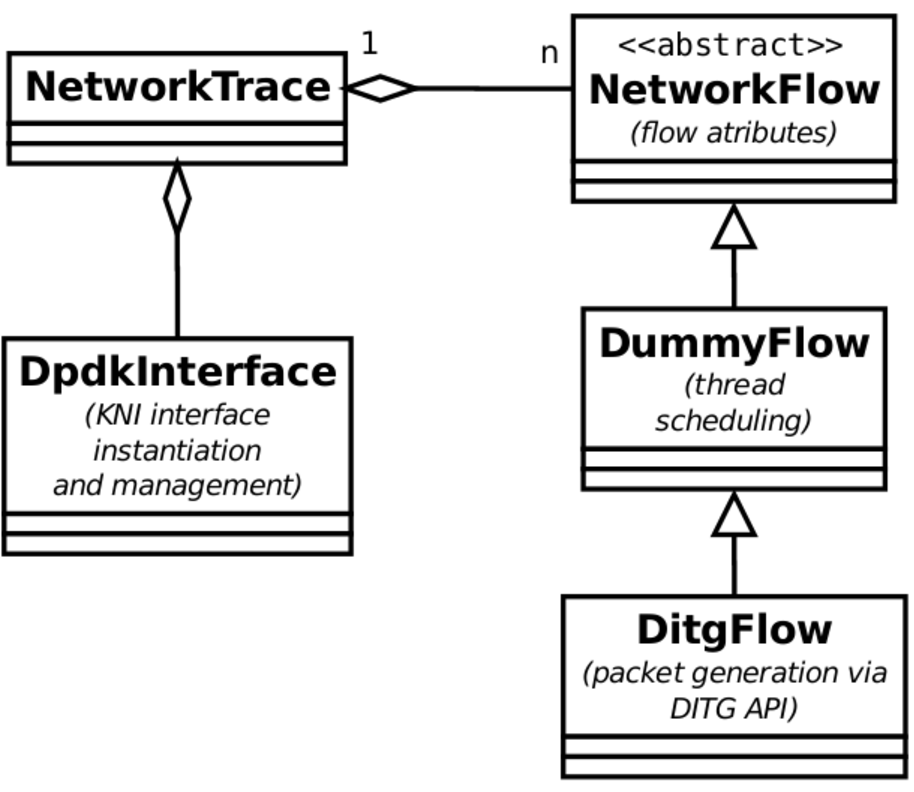
\includegraphics[height=2.0in]{figures/ch6/dpdk-interface.pdf}
    \caption{Usage of DPDK KNI interfaces.}
    \label{fig:dpdk-kni}
\end{figure}

\textbf{[A.4]} One possibility to improve the traffic generation performance issue DPDK Kernel NIC Interface (KNI interfaces) 2. DPDK KNI interfaces allow applications from the user’s space to interact with DPDK ports. In this way, we may achieve a faster packet processing.

\subsection{Multi-thread C++ Sniffer}

\textbf{[A.5]} Implementing a C/C++ multi-thread sniffer will improve the processing time of packets. 



%%%%%%%%%%%%%%%%%%%%%%%%%%%%%%%%%%%%%%%%%%%%%%%%%%%%%%%%%%%%%%%%%%%%%%%%%%%%%%%
\section{Tool Support}

\subsection{Inter-packet times on TinsFlow}

\textbf{[B.1]} SIMITAR’s current implementation using libtins to generate the packets does not model inter-packet times. Modeling this feature will improve the scaling characteristics of libtins traffic.

\subsection{D-ITG, Ostinato and DPDK Flow Generators: DitgFlow, OstinatoFlow, DdpkFlow}

\begin{figure}[!ht]
    \centering
    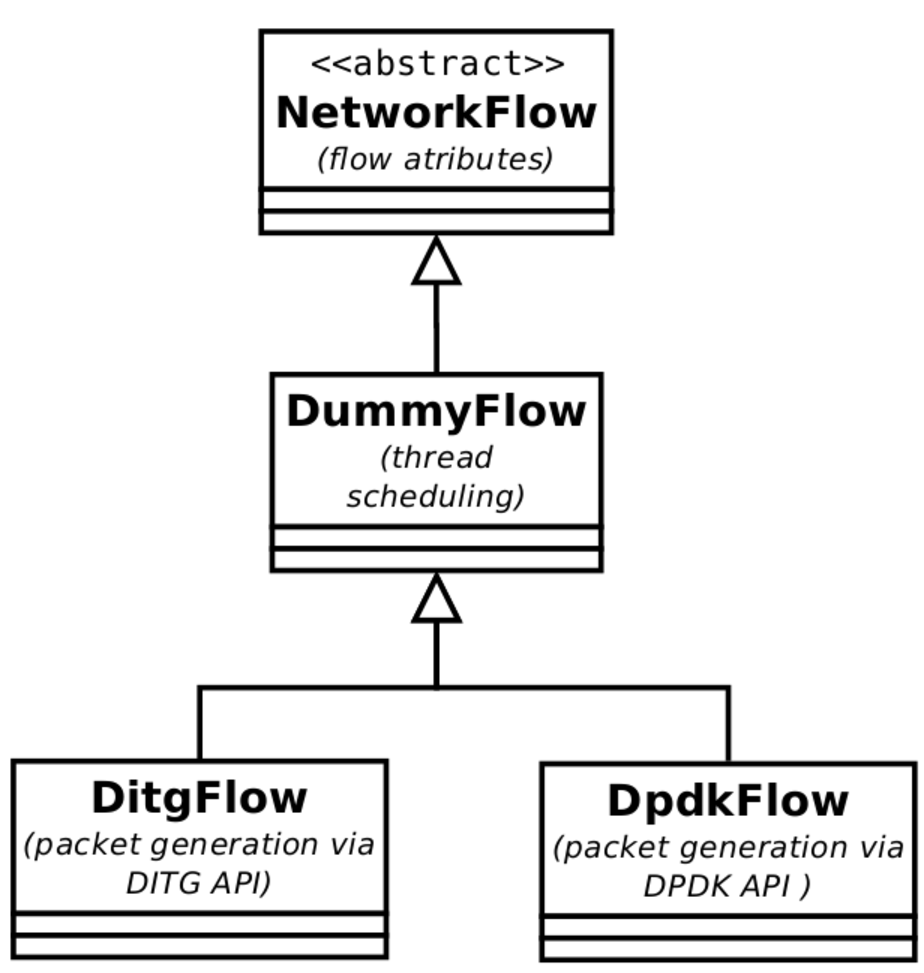
\includegraphics[height=2.0in]{figures/ch6/dpdk-flow}
    \caption{DddkDlow and DitgFlow}
    \label{fig:dpdk-flow}
\end{figure}


\textbf{[B.2-4]} Expand SIMITAR to other traffic generator tools(figure~\ref{fig:dpdk-flow}). D-ITG offers many stochastic functions for customization of inter-packet times, Ostinato provides a rich set of headers and protocols, and DPDK a high performance on packet generation. Each tool can offer a different result on traffic generation,  each with their benefits. 

\subsection{ZigBee protocol Support}

\textbf{[B.5]} Finally, to apply SIMITAR on IoT scenarios, we will have to provide support for new protocols, such as ZigBee\cite{zigbee}.



%%%%%%%%%%%%%%%%%%%%%%%%%%%%%%%%%%%%%%%%%%%%%%%%%%%%%%%%%%%%%%%%%%%%%%%%%%%%%%%
\section{[C] Calibration}


\subsection{ \texttt{min\_time}}

\textbf{[C.1]} Calibrate the constant \texttt{DataProcessor::min\_time}: smallest time considered for inter-packet times. We use this value to avoid inter-packet times equals to zero due to the sniffer resolution. Today, this value is $5e^{-8}$.

\subsection{\texttt{min\_on\_time}}

\textbf{[C.2]} Calibrate the constant \texttt{DataProcessor::m\_min\_on\_time}: this value controls the small ON time that a file can have. It can change the generated traffic precision. Currently, this value is $0.1$s. 

\subsection{\texttt{session\_cut\_time}}

\textbf{[C.3]} Calibrate the constant \texttt{DataProcessor::m\_session\_cut\_time}. \texttt{calcOnOff} uses this value to defines whatever a file transference still active or has ended.  This constant affects performance on traffic realism. 



%%%%%%%%%%%%%%%%%%%%%%%%%%%%%%%%%%%%%%%%%%%%%%%%%%%%%%%%%%%%%%%%%%%%%%%%%%%%%%%
\section{New Components}


\subsection{Traffic Measurer}

\begin{figure}[!ht]
    \centering
    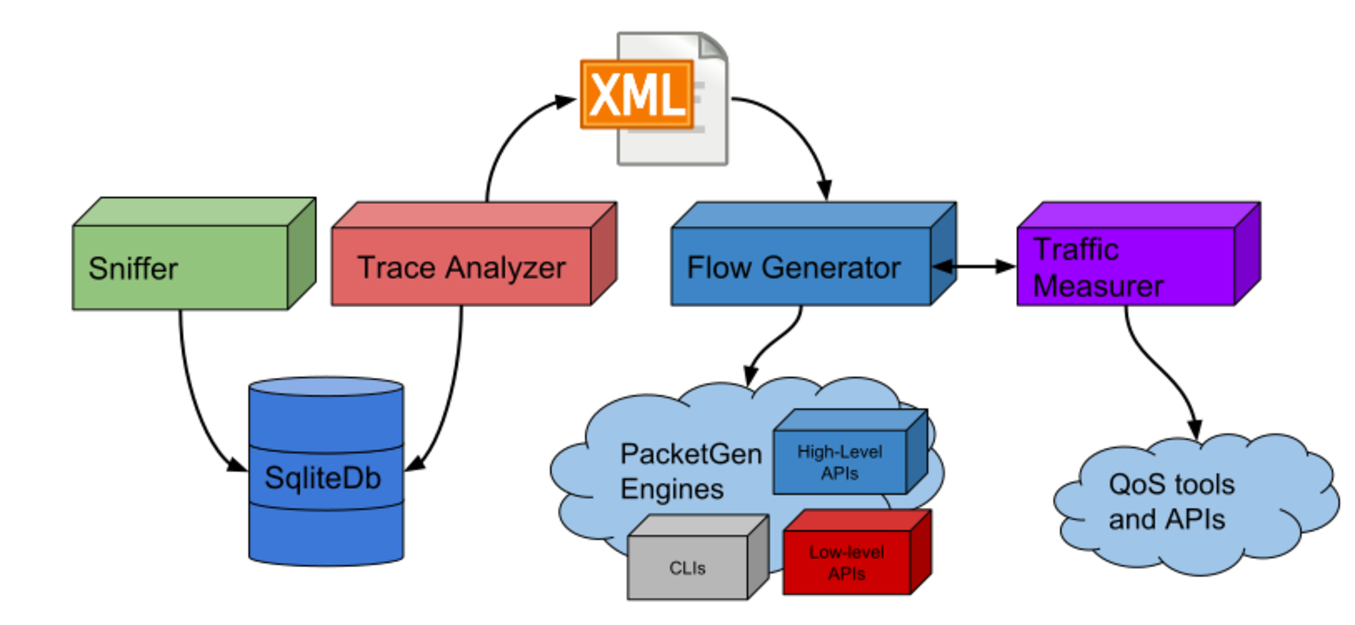
\includegraphics[height=2.0in]{figures/ch6/traffic-measurer}
    \caption{Component for measurement of traffic statistics: packet-loss, throughput, available bandwidth, delay, RTT, and jitter.}
    \label{fig:traffic-measurer}
\end{figure}


\textbf{[D.1]} Develop a component able to extract useful QoS information from the generated traffic is essential on the applicability and utility of our tool(figure~\ref{fig:traffic-measurer}). This can be done by:
\begin{itemize}
\item Counting the transmitted and received packets, to estimate the \textit{\textbf{packet-loss}} and the \textit{\textbf{throughput}}.
\item Apply techniques of passive measurement of \textit{\textbf{available bandwidth}}, such as the ones used by Pathload\cite{web-pathload} and pathChirp\cite{pathchirp-paper}\cite{web-pathchirp}.
\item Create signaling channels to estimate the \textit{\textbf{delay}}, \textit{\textbf{RTT}} and \textit{\textbf{jitter}}. 
\end{itemize}

\subsection{Pcap files crafter}

\begin{figure}[!ht]
    \centering
    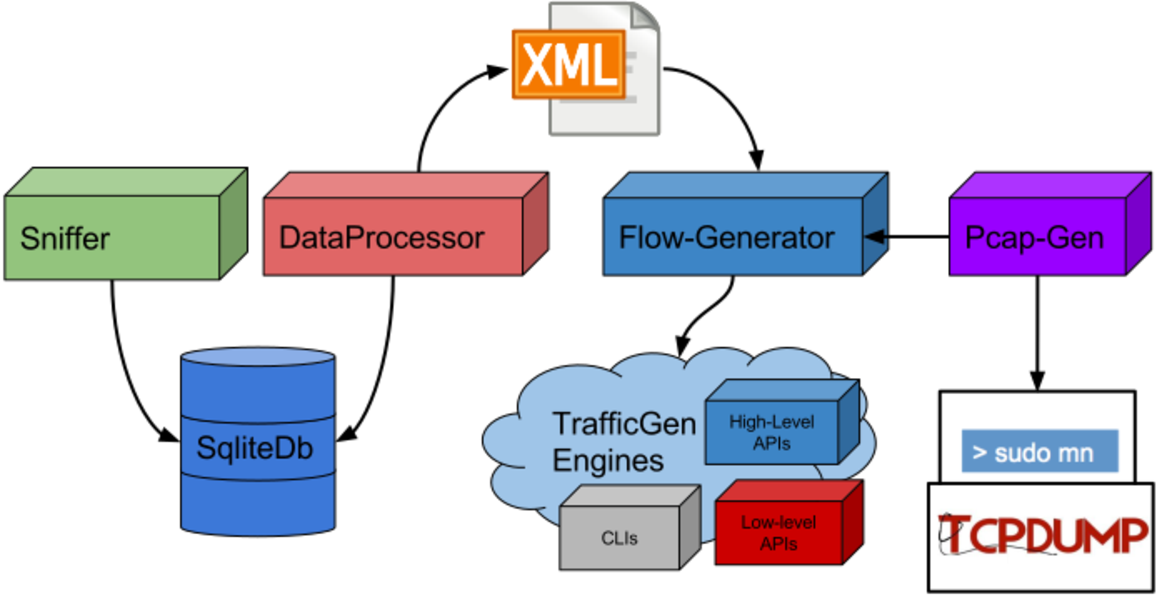
\includegraphics[height=2.0in]{figures/ch6/pcap-gen}
    \caption{Using SIMITAR for generation synthetic \textit{pcap} files, CTD files: a component schema}
    \label{fig:pcap-gen}
\end{figure}


\textbf{[D.2]} PcapGen, a pcap generator tool: Create a component capable of generating synthetic pcap files, using Compact Trace Descriptors files, using TCPDump\cite{web-tcpdump} and Mininet\cite{web-mininet}.  We present a diagram of this idea in figure~\ref{fig:pcap-gen}. This expansion would enable SIMITAR to work as trace library for pcap-based benchmark tools.

\subsection{Python/Lua Flow Generator}

\textbf{[D.3]} Currently, SIMITAR only enables the programming of flow traffic generation in C++. Adding Python and Lua support for the Flow Generator component, we can allow expansion for Python/Lua traffic generation APIs (such as Ostinato and MoonGen APIs), without creating C++ wrappers. 


%%%%%%%%%%%%%%%%%%%%%%%%%%%%%%%%%%%%%%%%%%%%%%%%%%%%%%%%%%%%%%%%%%%%%%%%%%%%%%%
\section{New Research Topics}


\subsection{Automated Selection of Inter-packet times models 2.0}

\textbf{[E.1]} Expand our work made on the validation of information criteria on the automated selection of stochastic models. 
\begin{itemize}
\item A deeper analysis of the impact on the maximum likelihood method in comparison to the others;
\item An analysis of the effectiveness of each parameterization method, and the best performance of each metric of quality measurement: correlation,  mean inter-packet time and Hurst exponent; 
\item Use of new stochastic methods functions, such as Log-Normal, Gamma, Poison, Binomial, Beta, and Chi-squared;
\item Use of Markovian-chain and Envelope processes;
\item Use other information criteria, such as AICc, MDL, nMDL\cite{information-criteria} and DIC\cite{dic-paper}.
\end{itemize}

\subsection{How how to craft malicious flows?}

\textbf{[E.2]} Research features used on by intrusion detection and intrusion prediction systems, and develop a method to mimic malicious flows, creating a "MaliciousFlow" model. At the same time, improve and evolve the current flow modeling, to ensure regular flows are not labeled as malicious flows by the same systems.  In that way, SIMITAR will be able to craft malicious traces, an important achievement on network security research.

\subsection{Envelope and Markovian-based traffic models}

\textbf{[E.3-4]} Evolve SIMITAR traffic model, and try the application of  Markovian and Envelope processes on the modeling of inter-packet times and ON/OFF times.
 
\subsection{ Fractal and multi-fractal modeling: models, Hurst exponent and  Hölder exponent.}

\textbf{[E.5]} Another proposal is to deepen the studies on Fractal and multi-fractal modeling. 

\begin{itemize}
\item Study a larger set of fractal models, including the above-mentioned Envelope and Markovian processes.  
\item Study the Hölder exponent\cite{holder-exponent}, a generalization over time of the Hurst exponent. 
\item Study the viability of parameterizing a process to have a specific value of Hust exponent. In other words, have the Hust exponent as a constraint for the model.
\end{itemize}

\subsection{Hurst-exponent feedback control system for ON/OFF times}

\begin{figure}[!ht]
    \centering
    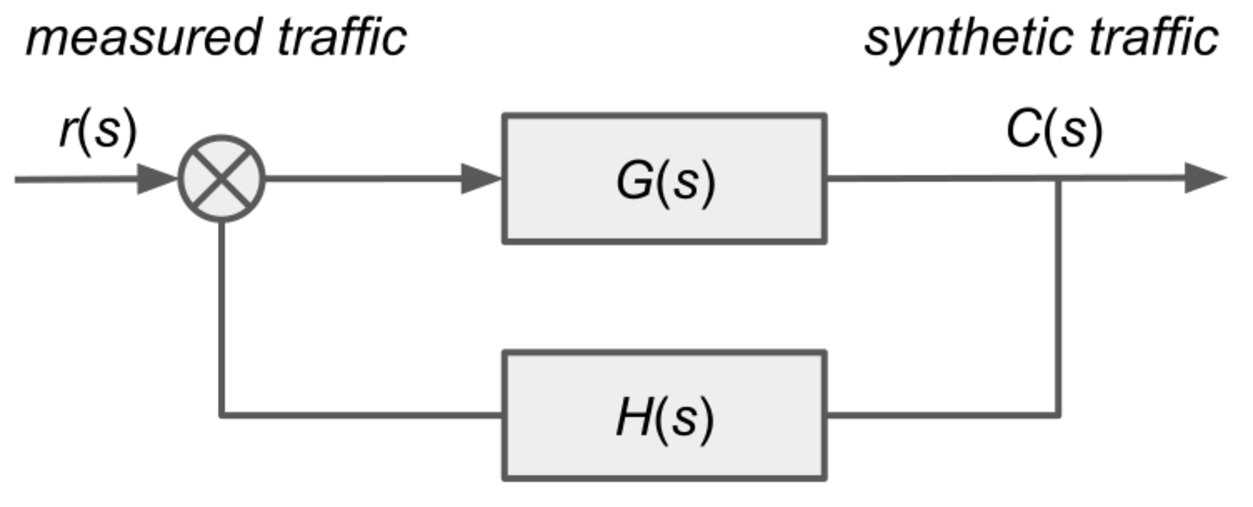
\includegraphics[height=2.0in]{figures/ch6/control-system}
    \caption{Schematic of a feedback control system applied on synthetic traffic generation.}
    \label{fig:control-system}
\end{figure}

\textbf{[E.6]} Study the viability of the application of a feedback system to control the parameters of the synthetic traffic; for example, Mean inter-packet time and Hurst Exponent(figure~\ref{fig:control-system}).

\subsection{Traffic generation based on Generative Adversarial Networks (GANs)}

\textbf{[E.7]} Other promising technology on controlling features can be the usage of Generative Adversarial Networks, also called GANs\cite{gans-paper}. This is a type of neural network used usually used on image synthesis, as we can see in figure~\ref{fig:gans-example}. We could apply the GAN to generate matrixes of features: inter-packet times, flows, protocols, packet sizes and so on(figure~\ref{fig:color-maps}).  Then, apply this matrix of features to synthesize network traffic. 

% GANs example
\begin{figure}[!ht]
    \centering
    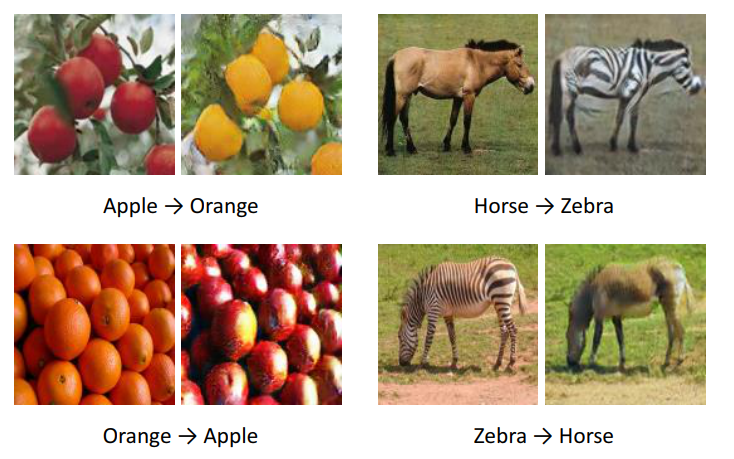
\includegraphics[height=2.0in]{figures/ch6/gans-example}
    \caption{Example of GANs application. GANs are commonly used for image synthesis. Source: \cite{gans-survey}. }
    \label{fig:gans-example}
\end{figure}

\begin{figure}[ht!]
    \centering
    \subfloat[\textit{skype-pcap}]{
        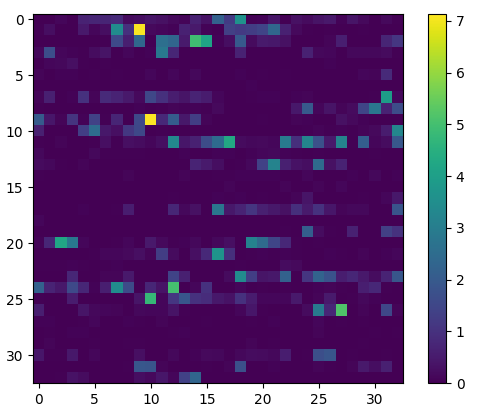
\includegraphics[height=40mm]{figures/ch6/colormap_skype.png}
    }
    \hspace{0mm}
    \subfloat[\textit{gateway-pcap}]{
        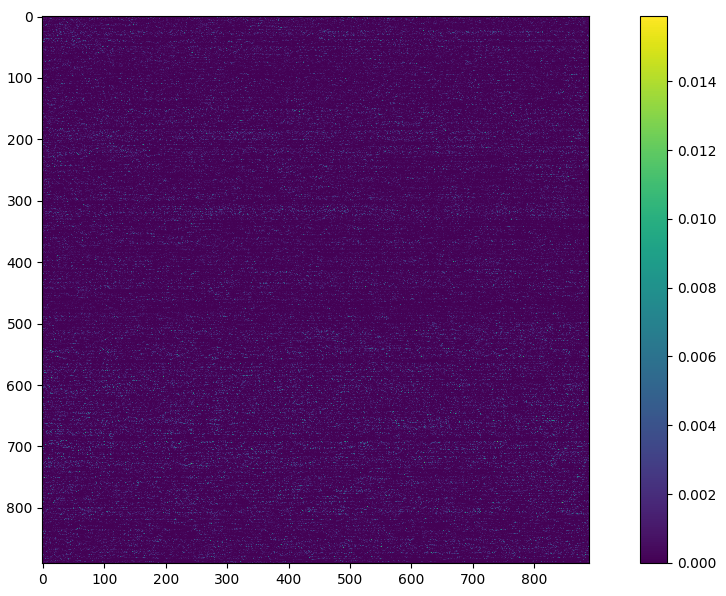
\includegraphics[height=40mm]{figures/ch6/colormap_gateway.png}
    }\\
    \hspace{0mm}
    \subfloat[\textit{firewall-pcap}]{
        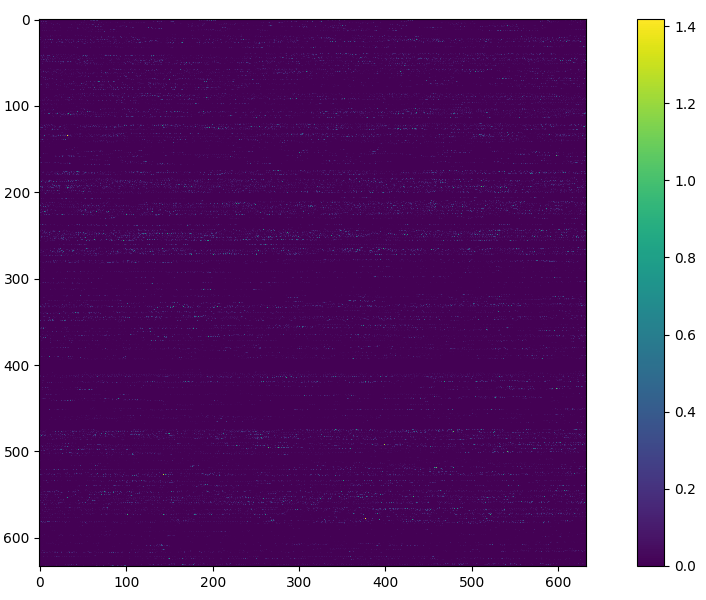
\includegraphics[height=40mm]{figures/ch6/colormap_firewall.png}
    }
    \hspace{0mm}
    \subfloat[\textit{wan-pcap}]{
        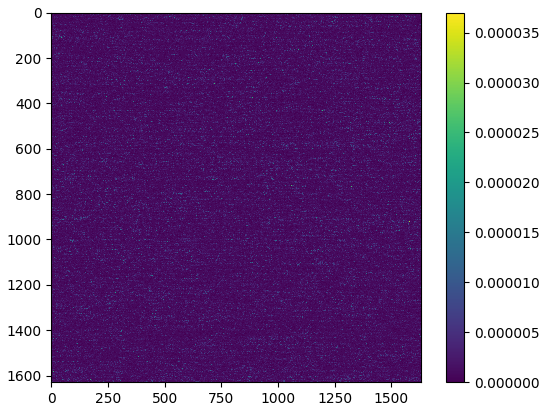
\includegraphics[height=40mm]{figures/ch6/colormap_wan.png}
    }
    \hspace{0mm}
    \caption{Color-map of inter-packet times from pcaps used on chapter~\ref{ch:modeling-evaluation}.}
    \label{fig:color-maps}
\end{figure}
%\clearpage

\subsection{ Realistic WAN, Wifi and IoT traffic}

\textbf{[E.8]} Expand the support for protocols and API of traffic generation to create synthetic traffic in different environments:
\begin{itemize}
\item Using DPDK, and improving the processing performance, we want to recreate WAN synthetic traffic. 
\item Support for new protocols, such as IEEE 802.11 (Wifi) and ZigBee, to create synthetic Wifi and IoT traffic.
\end{itemize}

\subsection{SIMITAR vs Harpoon}

\textbf{[E.9]} A "trial by fire", after improving the tools with these new features, compare the performance on realism and throughput of SIMITAR and Harpoon.

\subsection{How well traffic generators simulate reproduce stochastic processes?}

\textbf{[E.10]} A parallel research topic. Evaluate how close traffic generators that use the stochastic process to model inter-packet times, can reproduce the theoretically expected values. 

\subsection{Traffic Generator Tools Survey}

\textbf{[E.11]} The idea is to consolidate the already collected knowledge on traffic generators (chapter~\ref{ch:literature-review} and appendix~\ref{ap:traffic-gen-survey}), with other topics of relevance in these subjects, inspired in the same structure used by other surveys.